%%%%%%%%%%%%%%%%%%%%%%%%%%%%%%%%%%%%%%%%%%%%%%%%%%%%%%%%%%%%%%%%%%%%%%%%%%%%%%%%%%%%%%%%%%%%%%%%%%%%%%%%%%
%%													%%
%% 	BAKALÁŘSKÁ PRÁCE - Začleňování geografických datových sad do OpenStreetMap			%%
%% 				 Martin Jákl								%%
%%													%%
%% pro formátování využita šablona: http://geo3.fsv.cvut.cz/kurzy/mod/resource/view.php?id=775 		%%
%%													%%
%%%%%%%%%%%%%%%%%%%%%%%%%%%%%%%%%%%%%%%%%%%%%%%%%%%%%%%%%%%%%%%%%%%%%%%%%%%%%%%%%%%%%%%%%%%%%%%%%%%%%%%%%% 

\documentclass[%
  12pt,         			% Velikost základního písma je 12 bodů
  a4paper,      			% Formát papíru je A4
  twoside,       			% Oboustranný tisk
  pdftex				    % překlad bude proveden programem 'pdftex' do PDF
]{report}       			% Dokument třídy 'zpráva'
%

\usepackage[czech, english]{babel}	% použití češtiny, angličtiny
\usepackage[utf8x]{inputenc}		% Kódování zdrojových souborů je UTF8
\PrerenderUnicode{č}

\usepackage[square,sort,comma,numbers]{natbib}

\usepackage{caption}
\usepackage{subcaption}
\captionsetup{font=small}
\usepackage{enumitem} 
\setlist{leftmargin=*} % bez odsazení

\makeatletter
\setlength{\@fptop}{0pt}
\setlength{\@fpbot}{0pt plus 1fil}
\makeatletter

\usepackage[dvips]{graphicx}   
\usepackage{color}
\definecolor{purple}{rgb}{0.4,0.0,0.4}

\usepackage{transparent}
\usepackage{wrapfig}
\usepackage{float} 

\usepackage{cmap}           
\usepackage[T1]{fontenc}    

\usepackage{textcomp}
\usepackage[compact]{titlesec}
\usepackage{amsmath}
\addtolength{\jot}{1em} 

\usepackage{chngcntr}
\counterwithout{footnote}{chapter}

\usepackage{acronym}
\usepackage{listings}
\lstset{language=XML,
  breaklines=true,
  literate={ý}{{\'y}}1,
  stringstyle=\color{blue},
  identifierstyle=\color{black},
  keywordstyle=\color{purple}\bf,
  morekeywords={osm,way,nd,tag}}

\usepackage[
    unicode,                
    breaklinks=true,        
    hypertexnames=false,
    colorlinks=true, % true for print version
    citecolor=black,
    filecolor=black,
    linkcolor=black,
    urlcolor=black
]{hyperref}         

\usepackage{url}
\usepackage{fancyhdr}

\usepackage[
  cvutstyle,          
  bachelor           
]{thesiscvut}


\newif\ifweb
\ifx\ifHtml\undefined % Mimo HTML.
    \webfalse
\else % V HTML.
    \webtrue
\fi 

\renewcommand{\figurename}{Obrázek}
\def\figurename{Obrázek}

%%%%%%%%%%%%%%%%%%%%%%%%%%%%%%%%%%%%%%%%%%%%%%%%%%%%%%%%%%%%%%%%%
%%%%%%%%%%% Definice informací o dokumentu  %%%%%%%%%%%%%%%%%%%%%
%%%%%%%%%%%%%%%%%%%%%%%%%%%%%%%%%%%%%%%%%%%%%%%%%%%%%%%%%%%%%%%%%

%% Název práce
\nazev{Začleňování geografických datových sad do OpenStreetMap}{ Integration of geographic datasets into OpenStreetMap}

%% Jméno a příjmení autora
\autor{Martin}{Jákl}

%% Jméno a příjmení vedoucího práce včetně titulů
\garant{Ing. Martin Landa, Ph.D.}

%% Označení oboru studia
\oborstudia{Geodézie, kartografie a geoinformatika}{}

%% Označení ústavu
\ustav{Katedra geomatiky }{}

%% Rok obhajoby
\rok{2016}

%Mesic obhajoby
\mesic{červen}

%% Místo obhajoby
\misto{Praha}

%% Abstrakt
\abstrakt 
{czech/ abstrakt}%
{english/ abstract}

%% Klíčová slova
\klicovaslova
{OpenStreetMap, import, IPR, python, GDAL}%
{OpenStreetMap, import, IPR, python, GDAL}

%%%%%%%%%%%%%%%%%%%%%%%%%%%%%%%%%%%%%%%%%%%%%%%%%%%%%%%%%%%%%%%%%%%%%%%%

%%%%%%%%%%%%%%%%%%%%%%%%%%%%%%%%%%%%%%%%%%%%%%%%%%%%%%%%%%%%%%%%%%%%%%%%
%% Nastavení polí ve Vlastnostech dokumentu PDF
%%%%%%%%%%%%%%%%%%%%%%%%%%%%%%%%%%%%%%%%%%%%%%%%%%%%%%%%%%%%%%%%%%%%%%%%
\nastavenipdf
%%%%%%%%%%%%%%%%%%%%%%%%%%%%%%%%%%%%%%%%%%%%%%%%%%%%%%%%%%%%%%%%%%%%%%%

%%% Začátek dokumentu
\begin{document}

\catcode`\-=12  % pro vypnuti aktivniho znaku '-' pouzivaneho napr. v \cline 

% aktivace záhlaví
\zahlavi

% předefinování vzhledu záhlaví
\renewcommand{\chaptermark}[1]{%
	\markboth{\MakeUppercase
	{%
	\thechapter.%
	\ #1}}{}}

% Vysázení přebalu práce
%\vytvorobalku

% Vysázení titulní stránky práce
\vytvortitulku

% Vysázení listu zadani
\stranka{}%
	{\sffamily\Huge\centering\ ZDE VLOŽIT LIST ZADÁNÍ}%
	{\sffamily\centering Z~důvodu správného číslování stránek}

% Vysázení stránky s abstraktem
\vytvorabstrakt

% Vysázení prohlaseni o samostatnosti
\vytvorprohlaseni

% Vysázení poděkování
\stranka{%nahore
       }{%uprostred
       }{%dole
       \sffamily
	\begin{flushleft}
		\large
		\MakeUppercase{Poděkování}
	\end{flushleft}
	\vspace{1em}
		%\noindent
	\par\hspace{2ex}
	{Chtěl bych poděkovat vedoucímu mé bakalářské práce, Ing. Martinu Landovi, Ph.D. ,
	za odborné rady a~pomoc při zpracování této práce. Dále bych chtěl 
	poděkovat své rodině za projevenou podporu a~trpělivost.}
}

% Vysázení obsahu
\obsah

% Vysázení seznamu obrázků
\seznamobrazku

% Vysázení seznamu tabulek
%\seznamtabulek

% jednotlivé kapitoly
\chapter{Úvod}
\label{1-uvod}

K projektu OpenStreetMap (OSM) jsem se dostal již před několika lety.
Zaujala mě možnost sám tvořit a upravovat \uv{mapu}.
Přidávat nové infomace ze svého okolí vlastním sběrem dat
a poté využívat takto vytvořenou mapu.

Postupem času jsem zjistil, co je, a co již není vhodné vkládat do mapy.
Když mi bylo na Fakultě stavební ČVUT v Praze nabídnuto vypracovat
bakalářskou práci na téma, které se dotýká problematiky datových importů OSM,
neváhal jsem. Nedávno totiž Institut plánování a rozvoje hlavního města Prahy
(IPR) uveřejnil všechna svá geografická data.
Tím vznikla možnost začlenit další vhodná data do projektu OSM.

Obsahem této práce je čtenáře nejprve seznámit s projektem
OpenStreetMap. Přiblížit mu vznik a vývoj projektu, užití a jeho licenci.
%%% ML: tato veta nedava smysl, co jste chtel presne rici
Jendá se o cíl, kam se budou importovat zpracovaná data z IPR.
Dále přiblížit problematiku datových importů do OSM a vysvětlit
pojem otevřená data (Open Data).

V praktické části navrhnout aplikaci v programovacím jazyce Python,
která by data poskytovaná IPR umožnila dávkově stáhnout a následně
importovat do pracovní geodatabáze PostGIS a popsat ovládání
vytvořené aplikace.

Následně provést rešerši zveřejněných dat IPR a porovnat je s daty,
která již jsou v OSM. Navrhnout, jaká data by byla vhodná importovat.
V průběhu práce konzultovat tento záměr s~komunitou OSM.
Nakonec vybraná data připravit k~importu z~geodatabáze PostGIS
do OSM.

\chapter{Teorie}
\label{2-Teorie}

\section{OpenStreetMap}
\label{OpenStreetMap}

\subsection{Vznik}
\label{vznik}
OpenStreetMap (OSM) je projekt, jež vznikl s cílem vytvoření a sběru 
volně dostupných geografických dat a následně jejich možné vizualizace
do topografických map. Projekt založil Steve Coast v červenci roku 
2004 v Anglii. Jako inspirace mu posloužil projekt Wikipedia.

Zprvu projekt využívalo jen pár nadšenců, postupem času ale získal
%%% ML: dvakrat "narustat" v jedne vete
projekt popularitu. S nárůstem počtu uživatelů narůstal i objem dat.
%%% ML: nejen kapacitu serveru, ale cele infrastruktury, resit dalsi otazky (bezpecnost a pod)...
Bylo tedy nutné zvyšovat kapacitu serverů. 

V dubnu roku 2006 byla založena nadace OpenStreetMap Foundantion pro financováni 
projektu jako takového (zaměstnanců, běhu serverů atd.). \cite{wikiOSM}


\subsection{Struktura dat}
\label{struktura dat}
OSM data jsou nyní ukládána v databázi PostgreSQL \footnote{viz \url{http://blog.cleverelephant.ca/2009/04/openstreetmap-moves-to-postgresql.html}}
%%% ML: tady to skoro vypada, ze jsou dava ve formatu XML ulozena
%%% primo v DB, cemuz tak ale neni; XML, resp. OSM je vymenny format
a jsou k dispozici ve formátu XML. Jeho výhoda je jasná 
struktura, snadná orientace v kódu pro člověka. Nevýhodou je ovšem větší objem
%%% ML: v jake slova smyslu (prvek ~ soubor) ???
dat, který lze ale snížit kompresí. Každý prvek má vlastní XML soubor. 

%%% ML: tady by se hodil vycet (itemize), chtelo by do vysvetlit, co je cesta a pod...
Třídy prvků v OSM jsou rozděleny na: uzel (node), cesta (way) a
relace (relation).

Příklad XML souboru pro cestu:

{\scriptsize
\begin{lstlisting}
<osm version="0.6" 
generator="CGImap 0.4.0 (32632 thorn-01.openstreetmap.org)" copyright="OpenStreetMap and contributors" attribution="http://www.openstreetmap.org/copyright" license="http://opendatacommons.org/licenses/odbl/1-0/">
   <way id="87249754" visible="true" version="2" changeset="34489106" timestamp="2015-10-07T11:52:41Z" user="Petr Dlouhý" uid="17615">
       <nd ref="1014526199"/>
       <nd ref="1014525941"/>
       <nd ref="1014526337"/>
       <nd ref="1014526022"/>
       <nd ref="1014526277"/>
       <nd ref="1014525984"/>
       <tag k="highway" v="path"/>
       <tag k="source" v="bing:ortofoto"/>
   </way>
</osm>
\end{lstlisting}
}


Uzel je definován jedinečným identifikátorem ({\tt node id=}). Jeho
%%% ML: dodat EPSG kod, vsechny souradnice jsou v jednom SRS...
souřadnice jsou ve WGS~84. Je také ukládána verze ({\tt version= }) a kdy
%%% ML: opet cestina (minimalne 2x "a")... preformulovat
byl do databáze přidán a v jaké změně to bylo provedeno ({\tt changeset=~}).
%%% ML: cely tento odstavec plati i pro dalsi elementy - way/area (?)
Dále k bodu je možné připojit různé atributy s klíčem a hodnotou ({\tt tag~k=~v=~}).

Linie je spojení dvou a více uzlů, dále má také svůj identifikátor ({\tt way~id=~}).
%%% ML: nejde o hlavicku, ale o xml atributy a tagy...
Hlavičku XML souboru má shodnou s bodem. Ale dále obsahuje také seznam id uzlů,
které ji tvoří. Liniím lze taktéž přiřadit atributy.

Linie lze ještě rozdělit na neuzavřené a uzavřené. Uzaveným liniím lze připojit
i atributy určené jen pro plochy. Například les ({\tt landuse=forest}).
%%% ML: veta nize - ?
V případě, když se přidá atribut, který je prot linie, ale chceme
ho použít pro plochy, musí se ještě přidat se atribut {\tt area=yes}.

Speciálním příkladem jsou relace ({\tt relation= }), do kterých lze zahrnout
jeden a více prvků. Lze do nich spojit prvky stejné, nebo odlišné třídy,
nebo i jiné relace. Například dálnice je tvořena několika liniemi (cestami), a ty
jsou zahrnuty do společné relace Dálnice D1. Nebo např. turistická trasa
(od~KČT) je relace sdružující jak linie (cesty, pěšiny) tak i uzly
(rozcestníky, vyhlídky, apod. ).

%%% ML: osm wiki zni familiarne, + reference v tomto pripade je lepsi
%%% hned za slovem, nemusim byt na konco odstravce
U atributů popsaných na osmwiki \cite{OSMfeatures} je vždy uvedeno, k jaké třídě je
vhodné a nevhodné je použít (dle komunity uživatelů OSM). Pokud se stane, že je použit
%%% ML: to ???
na~jinou než povolenou třídu, nemusí to hlásit chybu, ale může být následně
%%% ML: viz kapitola?
problém v některých vykreslovačích. 

\subsection{Změna licence}
\label{změna licence}

%%% ML: Původně vs. původní data...
Původní data OSM a generované grafické dlaždice
byly na distribuovány pod licencí
Creative~Commons~AllributionShare~Alike 2.0 (CC~BY~SA~2.0).

Tato licence umožňovala užití (distribuci ale i editaci) díla pod podmínkou,
že bude uveden zdroj OpenStreetMap.org ve viditelné části
vytvořených mapových dlaždic \cite{OSMlicence}.

  \begin{figure}[hbt]
    \centering
      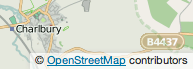
\includegraphics{./pictures/attribution_example.png}
      \caption{Příklad umístění licence}
      \label{fig:attribution_example}
  \end{figure} 

%%% ML: duvod zmeny ?
V roce 2012 byla licence publikovaných dat změněna na Open Data Commons
Open Database Licence (ODbL).
Tato změna licence přinesla problém
s~daty, které byly poskytnuty projektu v předchozí licencí
(CC~BY~SA~2.0). Bylo nutné se dotázat každého z dřívějších
přispěvatelů dat, ať už právnických osob, tak i fyzických osob, jestli
%%% ML: slo o to, zda souhlasi aby jejich prispevky byly poskytovany
%%% pod novou licenci, veta to naznacuje, ale je nepresna
s touto změnou souhlasí a je možné s jejich daty i s novou licencí
nakládat. U přispěvatelů, kteří nedovolili užívání jejich díla
%%% ML: co vymazat - jejich prispevky - preformulovat
pod novou licencí, nebo u těch, co se nevyjádřili, bylo nutné
%%% ML: chybi reference, co znamena zlomek?
z~databáze vymazat. Tato situace nastala pouze ve zlomku případů.
%%% ML: v jake mire? doplnit
Nejvíce tato změna licencí ohrozila data v zemích jako je Polsko a Nový Zéland.

%%% ML: proc tento dualismus?
V současnosti jsou tedy data OSM distibuována pod licencí ODbL a
generované grafické dlaždice pod licencí CC-BY SA 4.0
\cite {OSMlicenceIssue}.

\subsection{Licence ODbL}

%%% ML: preformulovat: Licence ODbl umoznuje...
Ve zkratce s daty pod licencí ODbL uživatel smí:
\begin{itemize}
    \item    kopírovat, distribuovat a užívat data
    \item    vytvářet nová data z původních
    \item    měnit původní data
\end{itemize}

%%% ML: preformulovat
S použitím ale uživatel musí ale uvést zdroj a licenci dat.
Dále uživatel souhlasí, že nová data vytvořená z původních dat budou sířena
také pod~licencí ODbL.
Podrobněji viz přesné znění licence na stránkách OpenDatabase.\footnote{\url{http://opendatacommons.org/licenses/odbl/1.0/}}


\subsection{Zdroje dat}
\label{Zdroje dat}

Jak bylo zmíněno, byla snaha, aby mapová data tvořili jedinci prvotním
sběrem dat, tj. měřením vlastními GNSS (GPS, Glonass) přijímači a
znalostí místních poměrů (uzavřené silnice, stezky atd.).  A takto
vzniklé dílo volně užívat k vlastním potřebám.  Komunita přispěvatelů se
zprvu pomalu, později poměrně rychle rozrostla a dnes čítá 3,7 milionů
registrovaných uživatelů s alespoň jednou vytvořenou změnou v OSM a
2,7 milionů účtů aktivních přispěvatelů.\cite{OSMstats}

Takto vzniklé mapové podklady byly velice vhodné i pro další projekt, dnes již
velice rozšířený a známý jako Geocashing (GC). Projekt GC začal mapové
podklady od OSM užívat a zároveň jeho uživatelé začali sami tvořit a
přispívat do OSM. 

Přispěvatelé dat do OSM musí respektovat licenci projektu OdbL.
Tudíž i jejich zdroj dat musí splňovat tuto licenci. Proto by měli
všechny svoje změny, které v OSM vytvoří, řádně ozdrojovat atributem
s~klíčem 
{\tt source}.
V případě vlastního sběru dat se vyplňuje hodnotou
{\tt source=survey} ,
popřípadně uvést zdroj, odkud čerpali. Pokud tuto povinnost poruší a
použijí zdroj, jež není kompatibilní s licenční politikou OSM, tak ostatní přispěvatelé do OSM tuto změnu, aby předešeli sporům, odstraní. V tomto případě dojde k odstranění celé sady změn, byť by v~ní byl pouze jeden prvek, jenž toto poruší.

%%% ML: nejen soukrome, ale i statni organizace, viz CUZK s RUIANem,
%%% OK mate to v dalsi odstavci
Druhým významným zdrojem dat jsou soukromé subjekty (společnosti).
Většinou jde o podkladové zdroje dat, například ortofoto. Pro obkreslování
silničních síti z~leteckých nebo satelitních snímků. V~jejich případě to
bylo řešeno písemným svolením, nebo smlouvou. Jako významným zdrojem byla
%%% ML: a ted uz neni...? Bing je spolecnost, nevlastni ji MS?
společnost Bing, jež nabídla k~dispozici letecké snímky většiny
obydlené pevniny. 

Třetím zdrojem dat a zároveň postupně dominujícím, co do jeho obsahu, jsou
%%% ML: ze -> produkované
datové sady ze státního sektoru. Tyto datové sady jsou nejvhodnějším zdrojem
%%% ML: proc ? vyargumentovat
dat.

\subsection{Vykreslovače}
\label{Vykreslovače}
Na hlavní stránce OSM (\url{http://www.openstreetmap.org}) je k dispozici mapová aplikace. Ta nabízí pět
„základních“ přednastavených vrstev vykreslených z~dat z OSM. Mapová
%%% ML: na cem je zalozen AJAX, kdyz uz to zminujete. Vysvetlit anebo odstranit.
aplikace OSM využívá knihovnu OpenLayers založenou na konceptu AJAX.
%%% ML: jde o EPSG:3857 - zminit, stejny souradnicovy system pouziva
%%% Google Maps a pod.
Pro snadné vykreslení dat do grafických dlaždic se používá Mercatorovo
zobrazení.

%%% ML: mozna dodat screenshoty do prilohy?
\begin{itemize}

  \item Standardní vrstva - vykresluje všechny prvky přiměřeně.
  \item Cyklomapa - vykresluje cyklostezky, výškopis. 
  \item Dopravní mapa - vykresluje silniční a železniční sítě.
  \item MapQuest Open - podkladová mapa právě pro potřeby 
    Geocaching.
    %%% ML: restaurace na prvni miste?
  \item Humanitární mapa, která vykresluje služby (restaurace, banky, muzea, 
  školy, kostely...)  a potlačuje ostatní prvky. 

\end{itemize}

%%% ML: kompozici? ruznych dat? dovysvetlit
Existují další stránky, jež se zabývají vlastní kompozicí a vykreslením
různých dat. Například mapu turistických a cyklistických tras vykresluje
pro celou Evropu mtbmap.\footnote{mtbmap.cz}

%%% priklad? mozna dodat hezky screenshot?
Zajímavými projekty jsou například ty, které k 2D mapě přidávájí „třetí“ rozměr a
vytvářejí tzv. 2.5D mapu. Většinou jde o 3D zobrazení budov, mostů (dle
atributů), popřípadě i stromů.

\section{Opendata}
\label{opendata}

%%% ML: od kud toto cerpate. Otevrena data (ala public domain) maji
%%% svuj puvod mnohem drive, v devadesatych letech...
Základní myšlenka otevřených dat vznikla v USA z iniciativy vlády Barracka Obamy.
%%% ML: nejen geograficka data
Tedy pokud vzniknou geografická data z veřejných peněz, měla by tedy být
%%% ML: tady neco tvrdite, ale nemate to podlozeno
přístupná veřejně. Mělo to kladný efekt na tamní ekonomiku. Díky tomuto byly
%%% ML: Landsat a SRTM jsou zverejnena jiz delsi dobu... to opravdu
%%% nesouvisi s vladou BO
zprvu k~dispozici satelitní snímky povrchu Země a digitální model terénu
s~rozlišením 30x30 m od NASA (pro pozdější vykreslení vrstevnic).

Tento trend se začal rozšiřovat zprvu do zemí západní Evropy,
%%% ML: druha cast vety nenavazuje na prvni, jake zeme, opet, nejaka
%%% reference?
jmenovitě Velké Británie, Francie či Německa, ale i jiné země mimo Evropu..

%%% ML: Fond se jmenuje Fond Otakara Motejla (opravdu jej zalozil on,
%%% nebyl zalozen na jeho pocet). Jednim z projektu fondu jsou prave
%%% Otevrena data
V ČR se tomuto věnuje fond Otevřená data\footnote{www.otevrenadata.cz}, který založil Otakar
%%% ML: Sociery? co Rekostrukce statu a pod.?
Motejl. Tento fond spolupracuje s nadací Sociery Fund Praha. V rámci
těchto uskupení je vyvíjen tlak na transparentnost veřejné správy a
zveřejňování smluv a dat
státních institucí, jelikož jejich získání a údržba byla placena
z~veřejných zdrojů.



\section{Importy}
\label{Importy}
Výraz import v tomto případě znamená začlenění většího množství datových sad
z~jednoho datového úložiště (databáze serveru) na jiný. Při velkých objemech dat
se využívá výkonu výpočetní techniky z důvodu její bezchybovosti, a také
z~důvodu časové náročnosti. Na člověku poté ale zbývá zvolit postup importu
a naprogramovat skript nebo program, podle něhož technika samotný proces
provede. 

Datové importy z veřejných databází do databáze OSM jsou velmi cenné. 
Otevřené geografické, ale i jiné, databáze státu a jeho veřejných institucí 
financovaných státem jsou komplexní. Komplexní v tom smyslu, že obsahují celistvý
soubor dat, protože je daná instituce vyžaduje ke svém chodu. Jistá nevýhoda tu 
ale může být, a to, že data nemusí být vždy úplně aktuální. Některá data mohou 
být sbírána a zveřejněna i s větším časovým odstupem.

V rámci České Republiky proběhlo již několik hromadných datových importů. Jak 
již bylo řečeno, větší časová náročnost zabere samotná příprava na import. A to
v~případě, importu do OSM. Nejen napsání skriptu, ale i nutná diskuze tohoto záměru
na~diskuzní konferenci Talk-cz. 

\subsection{Talk-cz}
\label{Talk-cz}
Tato diskuze probíhá přes posílání emailových zpráv do společné konference. 
Uživatelům chodí emaily z probíhající diskuze a pokud na nějaký chtějí reagovat,
tak pošlou email na adresu serveru, na kterém diskuze běží, a musí do Předmětu 
napsat Re: a předmět zprávy, na kterou reagují. Server tyto zprávy pomocí 
předmětu a času řadí. Diskuze je poté k dispozici na webových stránkách.\footnote{http://lists.openstreetmap.org/listinfo/talk-cz}

\section{IPR Praha}
\label{IPR Praha}
IPR Praha je zkratka názvu Institut plánování a rozvoje a hlavního města Prahy. 
Tento institut se věnuje urbanismu, architektury a rozvoje města Prahy. Hlavním
úkolem IPR je tvorba územního plánu Prahy a významným úkolem IPR je zajišťovat
zpracování geografických informací. Spravuje data a mapy města Prahy. Od roku 
2002 poskytuje na svých stránkách zdarma webové aplikace bez limitu využití. 
Po~rozvoji Pražského geoportálu došlo k jejich většímu využívání.  Na základě 
platných Pravidel pro poskytování dat a  výstupů z datových souborů a datového 
skladu Geografického byla od dne 1.~4.~2015 zveřejněny datové soubory a další 
webové služby. Tato data byla uveřejněna pod licencí CC-BY SA 4.0 \cite{IPR}
\subsection{licence CC BY-SA 4.0}
\label{licence CC BY-SA 4.0}
Licence CC BY-SA 4.0 je zde uvedena ve zjednodušeném znění.

"Uživatel s smí
\begin{itemize}
    \item   Sdílet - rozmnožovat a distribuovat materiál prostřednictvím jakéhokoli média v jakémkoli formátu
    \item   Upravovat - remixovat, změnit a vyjít z původního díla
\end{itemize}
pro jakýkoliv účel, a to i komerční.

Poskytovatel licence nemůže odvolat tato oprávnění do té doby, dokud dodržujete licenční podmínky.

Uveďte původ — Je Vaší povinností uvést autorství, poskytnout s dílem odkaz na licenci a vyznačit Vámi provedené změny. Toho můžete docílit jakýmkoli rozumným způsobem, nicméně nikdy ne způsobem naznačujícím, že by poskytovatel licence schvaloval nebo podporoval Vás nebo Váš způsob užití díla.

Zachovejte licenci — Pokud budete toto dílo upravovat, pozměňovat nebo na něj navazovat, musíte svoje odvozená díla vystavovat pod stejnou licencí jako původní dílo."

Podrobněji viz přesné znění na stránkách CraetiveCommmons.
\footnote{https://creativecommons.org/licenses/by-sa/4.0/legalcode/}


\section{PostgreSQL}
\label{PostgreSQL}
PostgreSQL je Opensource databázový systém, který je vyvýjen déle než patnáct
let. Za dlouhou dobu vývoje se stal robustní a také hojně využívaný.
Postupem času získal svou spolehlivostní silnou reputaci.
Lze s ním pracovat ve všech známých operačních systémech. 
...
\cite{PostgreSQL}

\subsection{PostGIS}
\label{PostGIS}
PostGIS je objektově-relační nadstavba databázové struktury PostgreSQL.
Rozšiřuje ji o funkce, které umožňují geometrické operace s objekty v ní uložené.
Třídy prvků mohou být buď bod (point), linie (line) nebo polygon (polygon).
Dále je možné více prvků jedné třídy sdružit do multi-relace, 
to jest  multiPoint, multiLine, multiPolygon.
Geometrie prvku určuje jeho polohu v určité souřadnicové soustave, neboli 
kartografickém souřadnice. Dále určuje i kartografickou soustavu, ve které je 
jeho geometrie určena. Je tedy dále možné při známých transformacích mezi
soustavami provádět transformace souřadnic. Základní operace jako délka, obvod,
plocha, ale jsou zde i sofistikovanější funkce, které lze s objekty nebo i mezi 
objekty provádět.

Sotware PostGIS je šířen pod GNU General Public License (GPLv2) licencí.


\section{Python}
\label{Python}
Programovací jazyk Python vznikl v roce 1991. Navrhlo ho Guido van Rossum. 
Je vyvíjen jako open source projekt. Inspiroval se hlavně programovacím jazykem
ABS, který byl přímo vytvořen pro~výuku začatečníků v programování. Python je 
proto jeden z nejvýhodnějších programovacích jazyků pro začínající programátory,
ale i přesto ho lze použít pro~praktické programování. 

Jedná se tedy o jednoduchý programovací jazyk podporující různá programovací 
paradigmata, hlavně objektové, imperiativní, procedurální a omezené míře i 
fun- kcionální. Je multiplatformní, lze jej tedy použít na různých operačních 
systémech. Klade velký důraz na syntaxi psaného kódu, využívá hlavně prázdné 
znaky v~psaném kódu.  

Programy nebo skripty lze psát v textovém editoru, ale je vhodné použít 
standartu PEP~8, který kontroluje prázdné znaky a správnou strukturu skriptu. 

V současné době je vydána stabilní verze 3.5.7, která vůči předchozí verzi 2.x
mění některá, již "zažitá" syntaxe. Například nejviditelnější je změna funkce 
{\tt print } pro verzi 2.x stačilo  {\tt print 'Ahoj'}  a pro verzi 3.x je již
nutné string vložit do závorek  {\tt print('Ahoj')}  . Tyto dvě dnes používané
verze 2.x a 3.x jsou navzájem nekompatibilní.
\cite{python} 
\cite{wikiPython} 
  
  
\subsection{knihovna argparse}
\label{argparse} 
Knihovna argparse, jejíž autor je Tshepang Lekhonkhobe, je knihovna 
do~programovacícho jazyku Pyhon. Řeší konzolový vstup do aplikace a zpracovává 
ho pro další použití v programu.\cite{argparse}


\subsection{knihovna xmltodict}
\label{xmltodict} 
Tato knihovna umí číst soubory ve formátu XML a zpracovává je do snažší formy 
dat, která je jednodušší manipulaci pro samotný program. Data z XML zpracuje
do formy datové řady (array), kde každý člen této řady může být opět řada dat.\cite{xmltodict}

příklad parsování dat ve XML formátu

{\scriptsize
\begin{lstlisting}
<head>
  <many>ele1</many>
  <many>ele2</many>
</head>
\end{lstlisting}
}

Po otevření a parsování se v Python(u) provede příkazem.

{\scriptsize
\lstset{language=Python}
\begin{lstlisting}
with open('example.xml') as fd: 
  doc = xmltodict.parse(fd.read()) 
\end{lstlisting}
}

Objekt {\tt doc} má poté podobu.

{\scriptsize
\lstset{language=Python}
\begin{lstlisting}
OrderedDict([(u'head', OrderedDict([(u'many', [u'ele1', u'ele2'])]))]) }
\end{lstlisting}
}

V této datové řadě lze již snadno procházet. 

{\scriptsize
\lstset{language=Python}
\begin{lstlisting}
doc['head']['many'][0]
ele1
\end{lstlisting}
}


\subsection{knihovna GDAL/OGR}
\label{GDAL/OGR}
Jedná se o knihovnu pro práci s geografickými daty a umožňuje jejich čtení a zápis.
Je psána v programovacím jazyce C++. Je považován za jeden z hlavních 
open~source projektů a je hojně používán ve sféře GIS. Pracuje s vektorovými a 
rastrovými datovými formáty. Podporuje velkou škálu souborových formátů, a to 
pro vektorová data, ale i pro rastrová. Obsahuje databázi definic kartografických
projekcí používaných na celém světě a databázi jejich známých transformací. 
Umožňuje tedy komplexní operace s geografickými daty. \cite{GDAL}


\section{QGIS}
\label{QGIS}
QGIS je program vytvořen za účelem prohlížení a editace geografických dat.
Jedná se o Opensource software. Je tedy možné, aby na jeho vývoji spolupracoval
kdokoli. Je možné si vytvářit novou funkci, nebo přímo zásuvný modul do programu.
Je možné je psát v jazyce C++ nebo Python.
Tyto moduly si uživatelé mohou poté stáhnout a přidat do QGISu a využívat.
QGIS také umožňuje využívat konzolově jazyk Python. Je možné si tak vytvářet
vlastní jednoduché skripty v jazyce Python a spouštět je v QGISu.

Od svého vzniku bylo vydáno již spoustu verzí programu.
Dříve byly verze pojmenovávány podle planet, později podle jejich měsíců a nyní se dávají
jména německých měst. V současnosti (duben 2016) je k dispozici verze 2.14 Essen

\chapter{Praktická část}
\label{3-Praktická část}

\section{server PostGIS}
\label{server PostGIS}
V rámci této bakalářské práce s daty byla zřízena databáze PostGIS na školním
serveru. Do této databáze byla nahrána verze dat z OSM pro celou Českou
Republiku. Tyto data jsou každý den pravidelně aktualizována.
Data z OSM jsou do školní databáze nahrávána pomocí programu {\tt osm2pgsql.py}.\footnote{dostupné na http://wiki.openstreetmap.org/wiki/Osm2pgsql}
Ten nejprve stáhne aktuální data pro celou evropu a následně ořeže
jen na území ČR. 

Pro každou ze tří tříd z OSM je vytvořena samostatná 
tabulka. Pro uzly je vytvořena tabulka {\tt czech\_point}.
Pro~cesty z~OSM je vztvořena tabulka {\tt czech\_line} a pro plošné 
prvky (uzavřené cesty s atributy pro plochy) je vytvořena tabulka
{\tt czech\_polygon}.

Každý prvek má přiřazen, v rámci tabulky, jedinečné číslo {\tt PID}, 
dále je vytvořena geometrie a pak pro každý atribut je stejnojmený 
sloupce s~hodnotou. 
Například bod s atributem {\tt landuse = forest} má vse sloupci 
{\tt landuse} hodnotu {\tt forest}.

Dále tato databáze bude používána pro analýzu a úpravu dat z~IPR a
pro~import do~OSM.


\section{IPR data}
\label{IPR data}
IPR na svém webu od jara roku 2015 zveřejǔne data.
U všech zveřejněných dat, které jsou ve~vektorovém formátu jsou
možnosti souborvé formáty GeoJSON, DXF, GML nebo ESRI Shapefile.
Dále je na výběr mezi dvěma kartografickými zobrazeními S-JTSK nebo WGS 84.

Celkem IPR zveřejňuje 96 druhů datových souborů a ty jsou rozděleny
do~kategorii.\footnote{viz stránka IPR www.geoportalpraha.cz/cs/opendata}

Pokud není řečeno jinak, jedná se o data ve vektorové formě.
Těmito kategoriemi jsou:

\begin{itemize}
    \item   3D model - Obsahuje 3D modely budov a mostů v Praze a digitální
            model povrchu (DMP) a dále rastrově digitální model povrhu a
            terénu, absolutní a relativní výšky budov.

            Z těchto dat by se pro OSM dala využít poloha budov ze~soubru
            Budovy 3D. Budovy jsou ale již importovány ze zdroje RUIAN, takže
            již nejsou potřeba přidávat.

    \item   Digitální technická mapa Prahy - jsou zde k dispozici v vektorové
            podobě inženýrské sítě v Praze, technické budovy a hranice parcel.

            Do OSM se, možná zatím, nepřidávají inženýrské sítě. V tuto nyní
            lze do OSM přidávat zdroje veřejného osvětlení. Takže pokud by
            nějaky sbour obsahoval značky veřejného osvětlení mohlo by se tato
            data importovat do OSM. Hranice města Prahy a městských čístí již
            v~OSM je. Technické budovy by bylo možné použít jako zdroj
            pro budovucí aktualizaci OSM.

    \item   Doprava - obsahuje cyklistické trasy a značky, pěší trasy
            parkovací zóny, automaty, P+R parkoviště a mapy zon PID (vektor)

            Cyklysticé trasy v Praze by se mohli importovat ale jsou již velmi
            dobře zmapované samotnými uživateli. Dataset obsahuje bodové značky
            a z těch by se některé mohli importovat.
            V případě dat Cyklistická doprava - značky, byla data prohledána, dle IPR
            uváděné hodnoty {\tt 103} ve sloupci {\tt DRUH} pro Bikeshating, bohužel žádné
            takové hodnoty neobsahovaly. Import dat z této tabulky nebyl dál brán v potaz.
            Bylo by možné do OSM přidat parkovací zony (jako nový atribut u stávajících komunikací).
            Vhodná data jsou parkovací automaty a také P+R parkoviště.

    \item   Geologie - obsahuje vektorové mapy radonového nebezpečí. Tato data
            se do OSM nepřidávají.

    \item   Hluk - obsauhjí hlukové mapy a to ve dne a v noci v rasterové formě.
            Tato data se do OSM nepřidávají. Dále obsahuje i protihlukové bariéry,
            tyto data by bylo možné do OSM přidat.

    \item   Kvalita životního prostředí - Obsahuje dataset Oblasti svozu komunílního odbadu.
            Tyto data nejsou vhodná do OSM začlenit. Dále ale obsahuje dataset
            Odpadní Zařízení pro občany, a toto obsahuje informace o všech sběrnách v Praze,
            tedy tento dataset je vhodný pro import.

    \item   Mapové podklady - obsahuje klady mapových listů různých měřítek (1:500 až 1:10 000)
            Tyto data nejsou vhodná do OSM. Dále obsahuje i vrstevnice a to po
            5~m, 2~m a 1~m. Vrstevnice přímo OSM neobsahuje a ani sám nevykresluje.
            Je ale možné tyto data využít pro kompozice s OSM.\footnote{projekt mtbmap.cz nebo http://mapa.prahounakole.cz/}

    \item   Občanská vybavenost obsahuje pouze dataset Veřejné toalety.
            Tyto data by bylo vhodné do OSM přidat.

    \item   Ochrana přírody a krajiny, obsahuje data ochraná pásma památných stromů.
            Bohužel ne samotné stromy. Vhodná data jsou z datasetů Přírodní parky a
            Významný krajinný prvek - registrovaný. Z těchto datasetů by se mohly
            doplnit nebo aktualizovat data v OSM.

    \item   Ortofoto obsahují letecké snímky (rastr) Prahy až s rozlišením 5cm
            na~pixel jak ve~viditelném spektru světla tak i v infračerveném.

            Ortofoto jsou vhodná pouze jako podkladový zdroj,
            například pro mapovací aplikaci JOSM.

    \item   Ovzduší, obsauje vektorové mapy znečištění ovzduší a také
            zdoje znečištění. Tyto data se v OSM nemapuje, jediné co by se
            mohlo přidat do OSM jsou bodové zdroje, a to značkou pro komín.
            Dále v této kategorii jsou i Bonity a to z různých hledisek (ovzduší, osvit...).
            Tyto data nejsou vhodná pro OSM.

    \item   Platný územní plán. V této kategorii jsou datasety Veřejně prospěšných staveb
            (plošné, liniové a bodové). Dataset VPS obsahuje také infomace o P+R u stanic metra.
            Data jsou z územního plánu, a tedy nemusí být realizovány.
            Po prozkoumání aktuálních a porovnání s datasetem Záchytná parkoviště P+R,
            jsou již tyto záznamy obsaženy v datasetu Záachytná parkoviště P+R.

    \item   Socioekonomická data, obsahuje pouze vektorovou mapu ceny pozemků.
            Tyto data se do OSM neřidávají.

    \item   Technická infrastruktura - vodní hospodářství, obsahuje záplavová území
            Q20, Q50 a Q100 a uzemí zaplavené v roce 2013. Tyto data se do OSM
            nepřidávají. Dále v této kategorii jsou datasety Protipovodňové ochrany,
            jsou zde protipovodnové, dočasné, zdi. Je možné tyto zdi přidat,
            ale jelikož se jedná o dočasné překážky a to ještě jen v době akutní povodně,
            nemjí smysl je do OSM přidávat.

    \item   Urbanismus z této kategorie by se dalo pro OSM využít informace
            z~datasetu Stavební uzávěry - dopravní. Ale by bylo nutné udržovat
            aktuálnost infomací o plánovaných dopravních uzavírkách.
            Dále by se mohla do OSM přidat počet pater budov z datasetu
            Podlaživost.
\end{itemize}


\subsection{licenční problém}
\label{licenční problém}
Jak již bylo řečeno výše, IPR svá data zveřejnil a stále zveřejňuje pod licencí CC-BY SA 4.0 viz \ref{licence CC BY-SA 4.0}.

Jelikož jsou ale data OSM distribuována pod licencí ODbL,
době tvorby této práce, neumožňuje jejich začlenění do databíze OSM.

Licence ODbl je licence zaměřená na databáze. Zaručuje licencční 
ochranu databázi jako celku. 

Na některá data (informace), jako například místní názvy (ulice, ..)
se nemohou vzdathovat autorská práva. Nebo na infomace, která 
nevyžadovala žádnou kretivitu pro "vytvoření" . 

Vyžaduje ale vzdání se licenčních nároků 
na data, která tam uživatel přidal. V některých zemích, kde se nelze 
úplně vzdát autoriskcýh práv, vyžaduje jejich vzdání se na nejnižší 
možnou míru a také souhlasí, že nebude vymáhat svoje autorská práva.
\cite{ODbl}

..není možné začlenit data s licencí CCBYSA do databází OSM..(proč??)


IPR byl kontaktován, zdali by mohla být jeho data použita do import.
Dle vyjádření vyplinulo, že IPR by neměl problém s použitím svých dat, jelikož
jsou šířena pod myšlenkou opendata. Byla navrhnuta možnost udělit od IPR vyjímku
licenčního použití pro OSM, avšak toto by neřešilo problém, že by tato data byla
k dispožici z OSM pro koncové uživatele pod licencí ODbL. Tedy co by někteý
uživatel nemohl s daty, distribuovaných přímo od IPR, provádět mohl by si je
obstarat z databáze OSM a pod licencí, která by jeho aktivitu neomezovala.

Dle vyjádření se tato situace bude ze strany IPR řešit tak, že se změní 
licence u distribuovaných dat. Tato změna licencování se očekává 
v~několika měsících.


\section{IprDownloader}
\label{Iprdownloader}
Jak již bylo řečeno tak IPR distibuje svá data a datové soubory přímo na své 
stránce. Data tam jsou distribuována možností odkazů ke stažení nebo je
k~dispozici kanál ve formátu ATOM ({\tt http://opendata.iprpraha.cz/feed.xml}).
Pomocí něho se lze také dostat ke všem distribuovaným datům.

Jelikož by bylo zdlouhavé stahovat všechny tyto soubory ručně, proto byl
vytvořen program, který umožňuje stahování a import dat. Skript byl napsán
v~programovacím jazyce Python a využívá knihovny GDAL.

Je rozdělen na tři soubory 
{\tt , IprDownloader.py , IprBase.py} a {\tt IprPg.py}.


\subsection{{\tt IprDownloader.py}}
Na primární skript {\tt IprDowloader.py}, který parsuje vstupní údaje a
zpracovává je k~dalšímu použití ve sriptu, viz \ref{argparse} .
Těmito základními údaji jsou
({\tt ---alike, ---crs, ---format, ---outdir ---d}). Dalšími vstupními údaji mohou
údaje o databázi, kam se mají data importovat. Těmi to vstupy jsou
({\tt ---dbname ---dbschema ---dbhost ---dbport ---dbuser ---dbpassword}).

Skript hlídá vstupní formát kartografických souřadnic a pokud se neshodují
s~možnými, oznámí chybu o špatném vstupu. Pokud uživatel vloží kartografické
zobrazení ve formě EPGS kodu, program jej převede na jeho název.


\subsection{{\tt IprBase.py}}
Skript {\tt IprBase.py} definuje třídu {\tt IprDownloader} se všemy 
potřebnými funkcemi. Většina funkcí slouží pro otevírání, čtení a parsování
XML souborů, viz \ref{xmltodict} .
Obsahuje funkci pro hledání, která prochází všechny záznamy a 
porovnává, zda vstupní přibližný název je obsažen v názvu souboru dat. Poté 
najde odkaz na xml souboru a otevře jej. Následuje vždy čtení a parsování. 
Poté v naparsovaných udajích najde dle nastavení {\tt crc, format} správný soubor 
a stáhne jej do definovaného adresáře.


\subsection{{\tt IprPg.py}}
Skript {\tt IprPg.py } definuje třídou {\tt IprDownloaderPg }, která dědí 
všechny funkce od třídy {\tt IprDownloader } a definuje další funkce potřebné pro 
správný import stažených dat do databáze PostgreSQL. 
Přesněji stažený soubor zkontroluje, jestli není v kompresován v archivu 
{\tt *.zip} , jeslit ano, extrahuje ho do nové složky se stejným jménem jako
archýv ve stejném adresáři jako archiv. Následně složí string pro PostgreSQL 
ze~vstupních údajů. Pro soubory ve formátu ESRI Shapefile opravý definici 
kartografického zobrazení uloženou v souboru {\tt *.prj }. 


\section{Ovládání}
Při pouhém spuštění skriptu vypíše všechna nalezená data, která IPR dává 
k~dispozici. Pro hledání a označení, která data se mají stánout slouží 
{\tt ---alike }. Za toto uživatel připojí slovo nebo frázi, jež chce v~datech
hledat. Pro~sousloví, které obsahuje mezeru, je vhodné jej umístit do uvozovek. 
Program rozlišuje velká~x~malá písmena a háčky a čárky.

příklad:

{\tt \$ iprdownloader.py ---alike 'Technická mapa'}
  

Dále jsou k dispozici nastavení.
\begin{itemize}
    \item kartografické zobrazení {\tt ---crs } . K dispozici jsou dvě
     (S-JTSK nebo WGS-84), respektive lze vkládat čtyři různé vstupy, protože 
     lze tyto kartografická zobrazení vložit i EPGS kody (5514 a 4326). 
     Přednastavené zobrazení je S-JTSK.
    \item datová formát souborů {\tt ---format} .
    
    Pro vektorové soubory je možné zvolit pro vektorová data:
        \subitem {\tt json }  JavaScript Object Notation
        \subitem {\tt dxf  }  AutoCAD DXF
        \subitem {\tt gml  }  Geography Markup Language
        \subitem {\tt shp  }  ESRI shapefile
        
    Je předdefinován formát {\tt shp} .
         
    Pokud uživatel chce stahovat rasterová data, je potřeba změnit předdefinovaný
    formát souboru na adekvártní rastrový formát např. ({\tt tif}) atd.
    
    \item adresu adresáře na místním počítači. Je předdefinován adresář 
    {\tt /data/} ve~složce, kde je uložen samotný program.     
\end{itemize}

Pro stažení dat stačí přidat parametr {\tt ---download} .

příklad:

{\tt \$ iprdownloader.py ---alike 'Technická mapa' ---crs 4326 ---format gmp ---outdir IPR}

Pro možnost stahované datové souboury importovat rovnou do databáze PostGIS, je 
minimálně nutné zadat název databáze {\tt ---dbname }. To v případě pokud je
databáze PostGIS umístěna v lokální síti. Pokud je databáze umístěna na jiném
serveru, je nutné zadat adresu {\tt ---dbhost} a port {\tt ---dbport} . Pokud je
ještě vyžadován autorizovaný přístup, použije se přístupové jméno {\tt ---dbuser} a
heslo {\tt ---dbpassword} . Je možné zvolit si schema v databázi {\tt ---dbschema} . 
Pokud je vložen název databáze, není již potřeba používat parametr {\tt ---download} .

Příklad:

{\tt \$ iprdownloader.py ---alike 'Technická mapa' ---dbname pgis\_osm\_jakl ---dbschema IPR ---dbhost geo102.fsv.cvut.cz  ---dbport 5432 } 
 

\section{Navržená data pro import}
\label{Navržená data pro import}

Po projití všech dat bylo vyhodnocena vhodna data pro začlenění do OSM. 
\begin{itemize}
    \item   Výstupy PID, obsahuje vstupy/výstupy z metra.
    \item   Odpadní zařízení pro občany, dle IPR obsahuje sběrny odpadu. 
    \item   Cyklistická doprava - značky, dle technické dokumentace by mělo 
            obsahovat bodové značky stojanů Bikesharing.
    \item   Veřejné toalety
    \item   Parkovací automaty
    \item   Záchytná parkoviště P+R
\end{itemize}

Všechna vybraná data byla pomocí IprDownloader.py stažena a naiportována 
do~školní databáze PostGIS. Poté byl program QGIS připojen na školní databázi.
Poté byla v programu QGIS pomocí SQL SELECTu filtrována data z aktuální
verze OSM na školním serveru a z každého SELECTu byla vytvořena nová tabulka 
v PostGIS databázi na školním severu. Data byla filtrována za použití doporučených
atributů na české osm wiki. \cite{OSMfeatures}

Tyto vhodná data byla projit a porovnána s aktuálním stavem v OSM.
Byly navrženy vhodné atributy který by se ze zdrojových dat daly naplnit.
Takto navržené data byla navržena na hromadná korespondenční konverzace talk-cz.


\subsection{Výstupy PID}
\label{Výstupy PID}
V datech od IPR bylo obsaženo celkem 353 záznamů. Jednalo se o vstupy/výstupy
z~metra (dveře, schodiště a výtahy).

V OSM databázi bylo hledání v tabulce {\tt osm.czech\_points} bylo použit
atribut
\begin{verbatim}
    railway = subway_entrance
\end{verbatim}
Vytvořená tabulka z dat OSM obsahovala 236 prvků.
Po porovnání dat bylo zřejmé, že nejvíce jsou v OSM zmapovány
výstupy v centru, kde jsou posuny v řádech decimetrů až metr. V okrajových
částech města nejsou zmapovány všechny výstupy nebo chybí výstupy pro celé
stanice. Protože body vstupů do metra jsou většinou součástí linií,
není vhodné body mazat a vytvářet nové. Bylo potřeba najít mezi stávajícími body
v~OSM a IPR adekvátní dvojce. To znamená, že se jedná o body, které reprezentují 
stejnou věc v~realitě.

Ani editaci stávajících není příliš přínosné, když všechny vstupy do metra jsou
minimálně 3 metry široké a všechny změny by byly v řádů cm až dm. 
Bylo by ale vhodné přidat vsupy do metra tam, kde nejsou v databázi OSM.
Jedná se o stanice metra Zličín, Luka, Kačerov, Rajská zahrada a Černý most. 
Celkem se tedy jedná pouze o 26 bodů, které by bylo snadnější přidat ručně, 
protože vstupy jsou dostatečně zmapované jen zde není na některém uzlu atribut {\tt railway~=~subway\_entrance}


\subsection{Odpadní zařízení pro občany}
\label{Odpadní zařízení pro občany}
Data od IPR obsahují seznam 36 směrných dvorů s velmi detailním popsání co 
jakou látku přijímá, otevírací dobu, zřizovatel. 

Z OSM z tabulky {\tt osm.czech\_point} byly prvky vyfiltrovány podle hodnot 
\begin{verbatim}
    amenity = recycling
    recycling_type = centre
\end{verbatim}    
Bylo nalezeno celkem 11 prvků, a z toho bylo 6 prvků z IPR ve vzdálenosti 
100 metrů od prvků z OSM. Těchto 6 prvků bude vhodné pouze přesunout. Zbylé 
prvky je nutné v databázi OSM nově vytvořit.

Z dostupných dat z tabulky byly navrženy tyto atributy: 
\begin{verbatim}
    amenity = recycling
    recycling_type = centre
    opening_hours =
    fee =
    operator = 
    source = 
    source:loc = IPR
\end{verbatim}
Tyto navržené atributy by se naplnily daty z tabulky dat z IPR.
Otevírací doba by byla vložena do {\tt opening\_hours~= }.
Hodnoty v tomto atributu by byly formátovány dle doporučeného formátování.\footnote{http://wiki.openstreetmap.org/wiki/Key:opening\_hours}
 U atributu {\tt fee~= }
bylo navrženo {\tt free of charge for the Prague citizens} , tedy zdarma pro občany Prahy.
Hodnota {\tt operator~= } by byla ze stejnojmeného sloupce z dat IPR.
Atribut {\tt source~= } by byl ze sloupce {\tt POSKYT }.

Dále byly navrženy atributy:
\begin{verbatim}
    recycling:paper = yes
    recycling:plastic = yes
    recycling:metal = yes
    recycling:wood = yes
    recycling: ... = yes
\end{verbatim}
Podle toho co zde lze recyklovat, dle hodnoty ve sloupci {\tt odpadprije }.


\subsection{Veřejné toalety}
\label{Veřejné toalety}
Datový soubor Veřejné toalety obsahuje jednu tabulku dat. V této tabulce je 
celkem 247 záznamů. U každého záznamu je uvedena lokalita, provozovatel. 
Dále je uvedena doba, po kterou je přístupný, zdali je nutné zaplatit poplatek,
jestli je bezbariérový a zdroj těchto dat.

Veřejné toalty byl v datech OSM byl vyhledán podle atribu
\begin{verbatim}
    amenity = toilets
\end{verbatim}

bylo zjištěno, toho času, 185 záznamů. Překrytí dat IPR a OSM bylo většinou
jeden bod z OSM a z IPR na tomto místě bylo, buď jeden ale posunutý, nebo
více bodů v okruhu několika metru. Na některých místech, převážně mimo centrum
Prahy a mimo linky metra, chyběli body veřejných toaletet úplně.
Bylo tedy vhodné stávající data doplnit data z IPR.

Na IPR dat z tabulky a základě doporučených atributů byly vybrány tyto atributy:
\begin{verbatim}
    acces = yes/permissive
    fee = no/yes
    wheelchair = yes/no
    opening_hours =
    operator =
    description =
    source = IPR
    source:location = IPR
\end{verbatim}
Pokud by hodnota byla {\tt fee~=~yes} připojila by se značka
\begin{verbatim}
    fee:price =
\end{verbatim}
hodnota by byla uvedena v Kč.

Hodnota u {\tt description~= } by byla hodnota ze sloupce {\tt lokalita} .
U atributu {\tt operator~= } byla navržena hodnota {\tt Hlavní Město Praha} ,
ale jen u~prvků, u~kterých je uvedeno HMP ve sloupci {\tt Operator}.
Tam kde není žádná hodnota, by se tento atribut nepřidal.


\subsection{Parkovací automaty}
\label{Parkovací automaty}
Soubor dat Parkovací automaty od IPR obsahovale celkem 452 záznamů parkovacích
automatů. Je zde uveden pouze TYP a Poskytovatel dat. Nelze tedy určit zdali
automat přijímá mimo, asi klasické, mince i bankovky, cizí měnu nebo i umožňuje
platbu platebními kartami.
Pro porovnání, byly vyhledány body z OSM s atributy:
\begin{verbatim}
    amenity = vendings_machine
    vending = parking_tickets
\end{verbatim}
Podle těchto parametrů bylo nalezeno pouze 8 bodových prvků v databázi OSM.
Pouze dva záznamy z OSM jsou v blízkosti k bodum z IPR.
Jeden je ve vzdalenosti okolo 5 metrů a druhý okolo 20 metrů. Nelze tedy určit
zda oba odkazují na stejný objekt nebo na dva různé.
Proto se původní prvky nebudou rušit. Nové prvky půjde zpětně rozlišit podle
atributu {\tt source:loc~= } .

U nově přidaných uzlů byly navrženy tyto atributy:
\begin{verbatim}
    amenity = vendings_machine
    vending = parking_tickets
    source = IPR
    source:loc = IPR
\end{verbatim}
Do hodnoty {\tt source~= } by byla použita hodnota ze sloupce {\tt POSKYT}) .
Hodnota u atributu {\tt source:loc~= } by byla použita {\tt IPR} .

\subsection{Záchytná parkoviště P+R}
\label{Záchytná parkoviště P+R}
Soubor dat Záchytná parkoviště P+R obsahoval 16 prvků.
V tabulce bohužel nejsou žádné jiné údaje, kromě polohy uložené v geometrii
a poksytovatel dat ve sloupci {\tt poskt}.

Z dat OSM byly vyhledány body pomocí atributu
\begin{verbatim}
    amenity = park_ride
\end{verbatim}
Tento atribut je stále ve fázi schvalování, tudíž nebyly nalezeny žádné záznamy.
Proto bylo vyzkoušeno hledání pomocí obecnějšího atributu
\begin{verbatim}
    amenity = parking
\end{verbatim}
Na území Prahy bylo nalezeno,toho času, 182 prvků.
Bylo vyzkoušeno hledání s přidaným atributem {\tt name~= }, který by obsahoval P+R.
Byl nalezen pouze jeden záznam.

Dále bylo vyzkoušeno hledání bodů s atributy 
\begin{verbatim}
    amenity = parking
    park_ride = yes
\end{verbatim}
Na území Prahy byl nalezen pouze jeden prvek.

Je tedy navrženo importovat všechny prvky z databáze IPR.
Navržené atributy jsou
\begin{verbatim}
    amenity = parking
    park_ride = yes
    source = HMP-URM
    source:loc = IPR
\end{verbatim}


\section{Návrhy z Talk-cz}
\label{Návrhy z Talk-cz}
Výše zmíněné návrhy byly takto zveřejněny a podrobeny diskuzi.

Výše zmíněná data byla zpracována v programu QGIS pomocí 
SQL. Byly vytvořeny, pro každý soubor, jedna tabulka připravená pro import.
Vždy pro každý atribut byl jeden sloupec (column) a příslužná hodnota atribut 
byla hodnota v tomto sloupci.
Každá tabulka mimo navržených atributů obsahovla sloupce s geometrii. 

Pro import  bude použit program osmosis.

Dále byly v diskuzi navrženo přidání výšky budov ze souboru dat Budovy 3D.

\subsection{Budovy 3D - výšky budov}
\label{Budovy 3D - výšky budov}
V diskuzi byla navržen import výšek budov {\tt building:height~= }
ze~sourbu dat Budovy 3D. 
A navržen atribut zdroje {\tt source:building:level~= }

..rešerše z OSM ..??

V souboru Budodvy 3D jsou uložny 3D polygonu tvoříci budovy.
Vždy polygony, které vytvářejí 3D model jedné budovy, 
mají stejnou bodnotu ve sloupci {\tt id\_bud} . 
Polygony se stejnou hodnotou {\tt id\_bud} lze dále rozdělit dle hodnoty 
ve~sloupci {\tt typ} na 
 
\begin{verbatim}
    dilci plocha stresni kruhove plochy
    komin
    sikma stresni plocha
    svisla obvodova stena
    vikyr_stresni nadstavba
    vytah_vetrani_klimatizace
    vodorovna stresni plocha
    vyznacena vez na strese
    zakladna vikyre, stresni nadstavby
    zakladova deska
 .. a další
\end{verbatim}

V 3D geometrii těchto polygonů budov jsou uloženy všechny (x,y,z) souřadnice 
vrcholů, jenž určují polygon. 

Pro nalezeni výšky budovy bylo dále pracováno pouze s polygony 
{\tt svisla obvodova stena}. 
Pro nalezení výšky každé stěny byly použity funkce pro hledání 
maximaní a minimální hodnoty z-ové souřadnice vrcholů.
Výška byla vypočtena jako jako rozdíl těchto hodnot. 

Přesněji bylo vypočtena takto {\tt ST\_ZMax(geom)-ST\_ZMin(geom) as height} 

Jelikož ale svislé stěny budovy může tvořit více než 4 polygony a 
ne všechny nemusí mít stejnou hodnotu (výšku), bula z těchto hodnot 
pro každou svislou stěnu vybrána maximální hodnota. Vždy v rámci jedné budovy. 
Tedy byla vybrána maximální hodnota výšky stěny budovy.


% Vysázení seznamu zkratek
%\begin{seznamzkratek}{ABCDE}

    \novazkratka{OSM}
		{OSM}
		{OpenStreetMap (\textit{Open Street Map})}

    \novazkratka{IPR}
	    {IPR}
        {Institut plánování a rozvoje hlavního města Prahy}

    \novazkratka{RUIAN}
	    {RUIAN}
        {Registr územní identifikace, adres a nemovitostí}

    \novazkratka{PID}
	    {PID}
        {Pražská integrovaná doprava}

    \novazkratka{KČT}
	    {KČT}
        {Klub českých turistů}

    \novazkratka{CC-BY-SA}
		{CC-BY-SA}
		{Uveďte původ-Zachovejte licenci (\textit{Creative Commons Attribution-ShareAlike})}

    \novazkratka{ODbL}
		{ODbL}
		{(\textit{Open Database License})}

    \novazkratka{GIS}
	      {GIS}
 	      {Geografický informační systém  (\textit{Geographic Information System})}

    \novazkratka{GNSS}
		{GNSS}
		{Globální družicový polohový systém (\textit{Global Navigation Satellite System})}

    \novazkratka{GPS}
		{GPS}
		{Globální polohovací systém (\textit{Global Positioning System})}

    \novazkratka{GLONASS}
		{GLONASS}
		{Glonass (\textit{Globalnaja navigacionnaja sputnikovaja sistěma})}

    \novazkratka{WGS 84}
		{WGS 84}
		{Světový geodetický systém 1984 (\textit{World Geodetic System 1984})}

    \novazkratka{S-JTSK}
		{S-JTSK}
		{Systém jednotné trigonometrické sítě katastrální}

    \novazkratka{GC}
		{GC}
		{Geocaching (\textit{Geocaching})}

    \novazkratka{SQL}
		{SQL}
		{SQL (\textit{Structured Query Language})}

    \novazkratka{XML}
		{XML}
		{Rozšiřitelný značkovací jazyk (\textit{Extensible Markup Language})}

    \novazkratka{GDAL}
		{GDAL}
		{Geoprostorová datová knihovna (\textit{Geospatial Data Abstraction Library})}

    \novazkratka{QGIS}
        {QGIS}
        {Quantum GIS}

    \novazkratka{JOSM}
        {JOSM}
        {Java OpenStreetMap Editor}


\end{seznamzkratek}


% Literatura
\nocite{*}
\def\refname{Literatura}
\bibliographystyle{mystyle}
\bibliography{literatura}


% Začátek příloh
%\prilohy

% Vysázení seznamu příloh
%\seznampriloh

% Vložení souboru s přílohami
%\chapter{Typy vykreslení OSM dat}
\label{vykresleni_dat}

\begin{figure}[H]
    \centering
    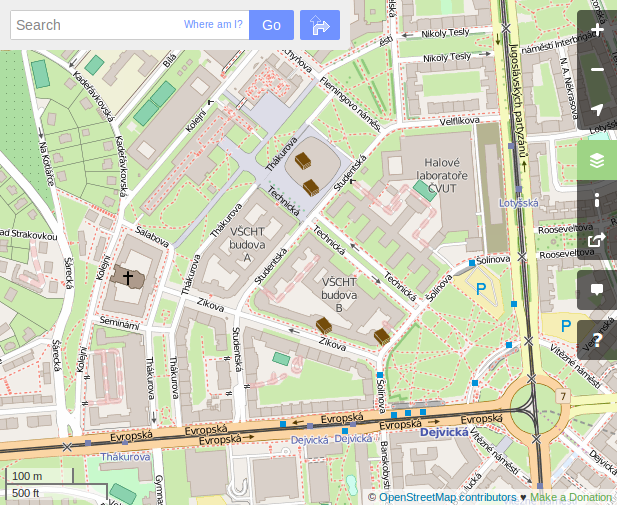
\includegraphics[width=11.5cm]{pictures/osm_standard.png} 
    \caption{Standardní mapa (Standard)}
    \label{fig:standard}
\end{figure}

\begin{figure}[H]
    \centering
    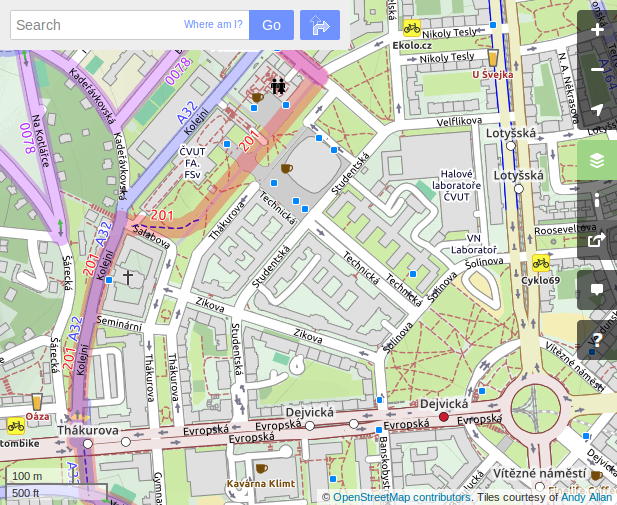
\includegraphics[width=11.5cm]{pictures/osm_cyclemap.png} 
    \caption{Cyklistická mapa (Cycle Map)}
    \label{fig:cycle}
\end{figure}

% new list

\begin{figure}[H]
    \centering
    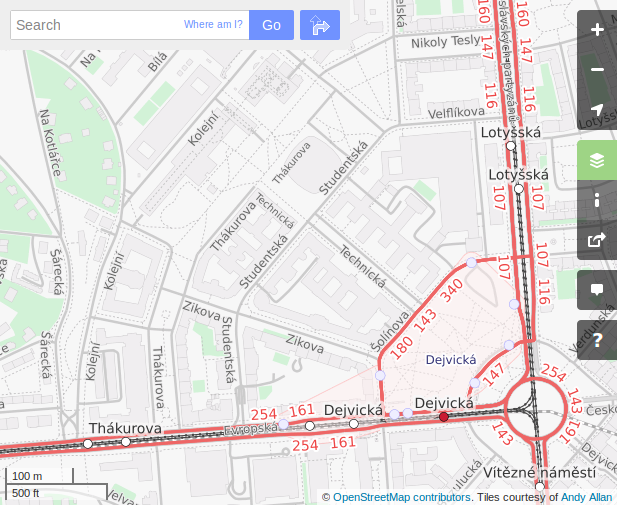
\includegraphics[width=11.5cm]{pictures/osm_transport.png} 
    \caption{Transport Map}
    \label{fig:transport}
\end{figure}

\begin{figure}[H]
    \centering
    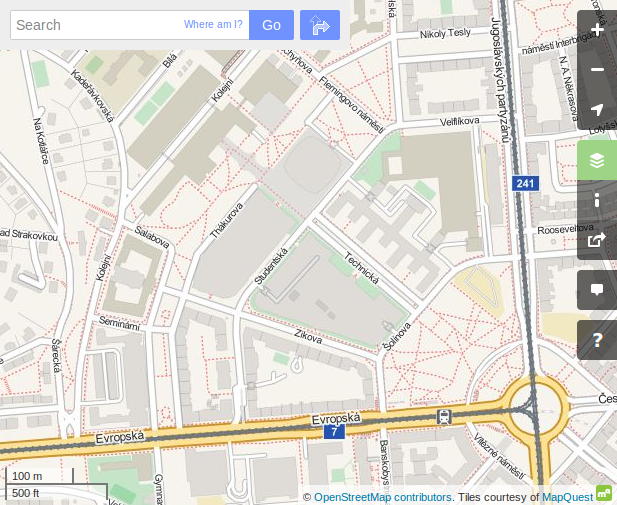
\includegraphics[width=11.5cm]{pictures/osm_mapquest.png} 
    \caption{MapQuest Open}
    \label{fig:mapquest}
\end{figure}

% new list

\begin{figure}[H]
    \centering
    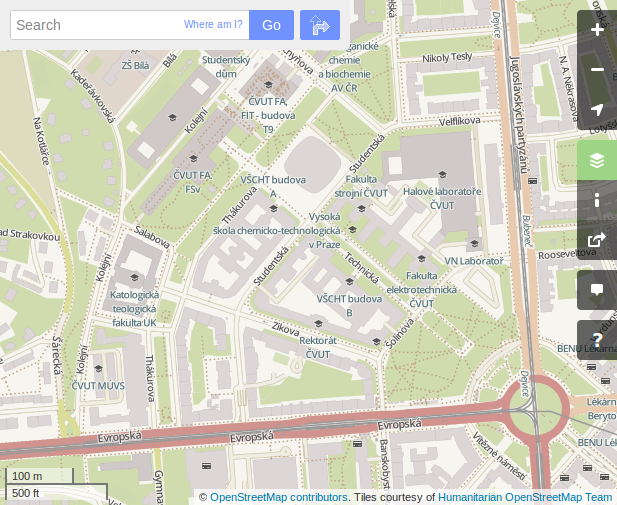
\includegraphics[width=11.5cm]{pictures/osm_humanitarian.png} 
    \caption{Humanitární mapa (Humanitarian)}
    \label{fig:humanitarian}
\end{figure}

\begin{figure}[H]
    \centering
    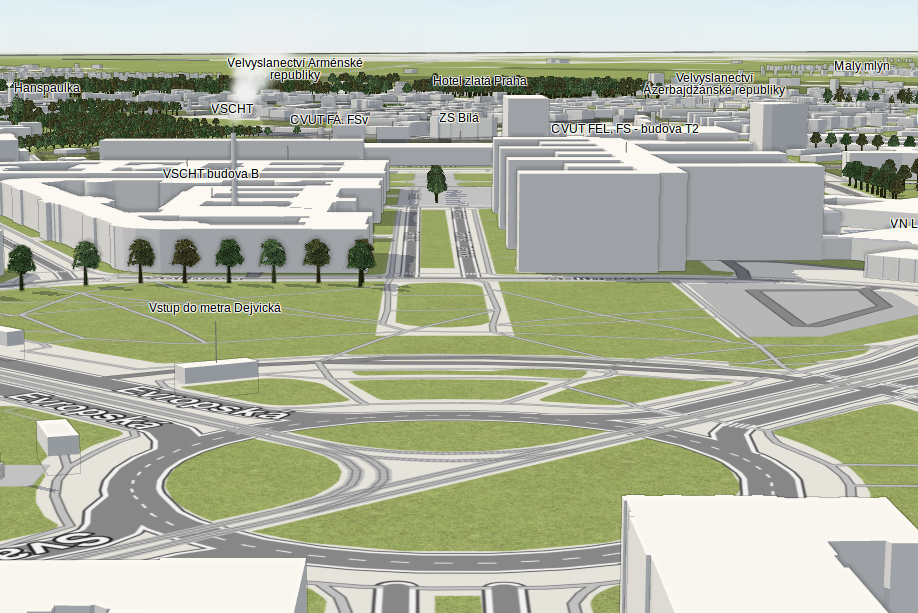
\includegraphics[width=11.5cm]{pictures/F4.png} 
    \caption{projekt F4 (zdroj \url{http://demo.f4map.com/}}
    \label{fig:F4}
\end{figure}

% new list

\chapter{Diagramy}
\label{digramy}

\begin{figure}[H]
  \centering
  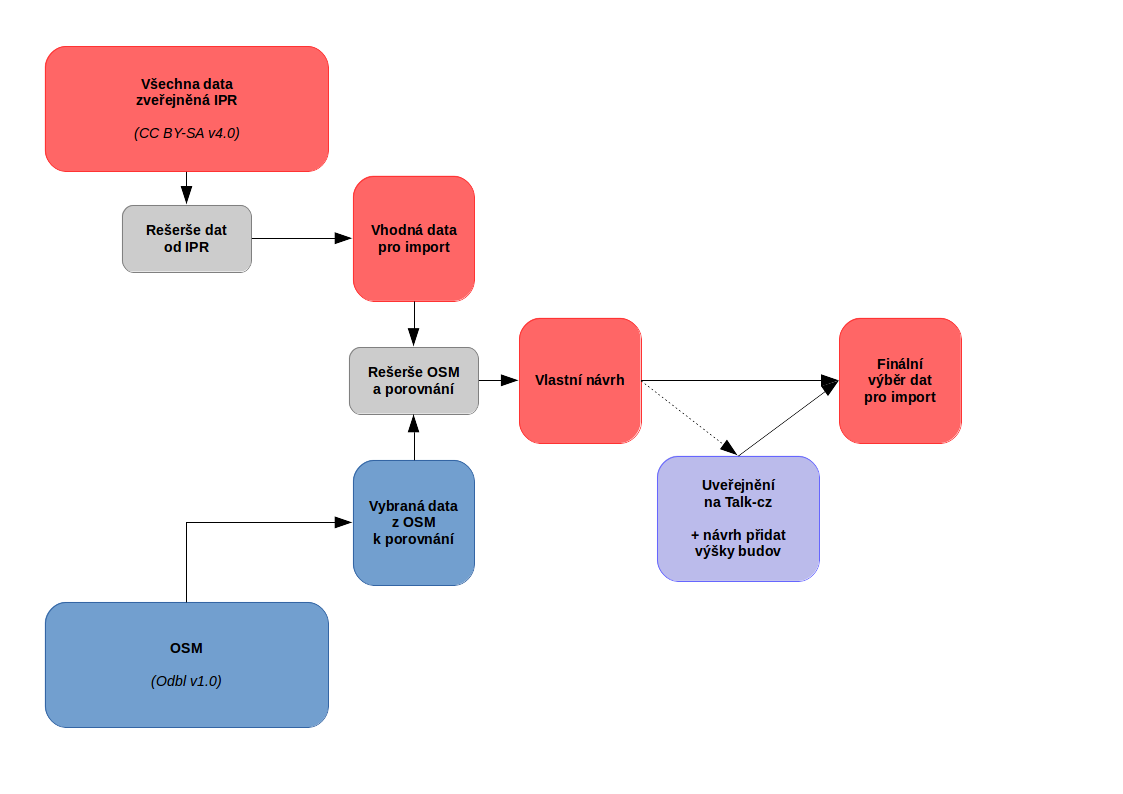
\includegraphics[scale=0.60,angle=90]{pictures/WorkFlow.png}
  \caption{Diagram postupu práce.}
  \label{fig:diagram_workflow}
\end{figure}

\begin{figure}[H]
  \centering
  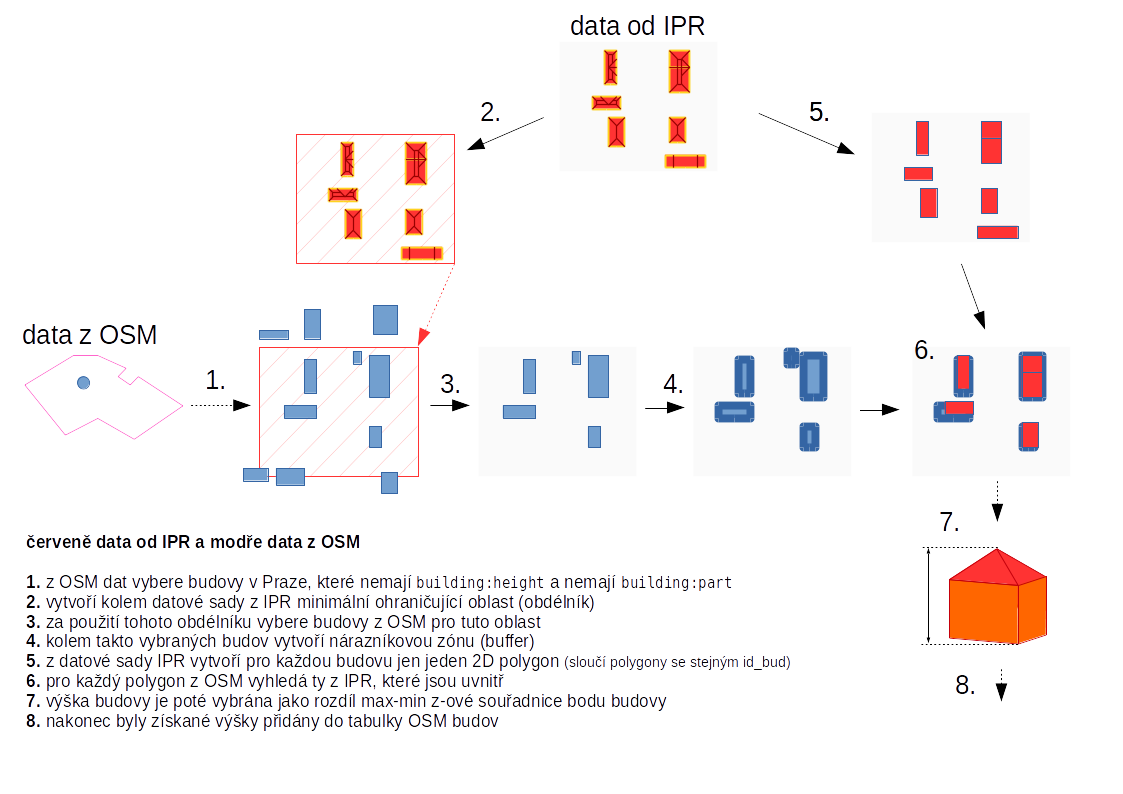
\includegraphics[scale=0.60,angle=90]{pictures/diagram_building_height.png}
  \caption{Diagram postupu práce pro získání výšky budov.}
  \label{fig:diagram_building}
\end{figure}

% new list

\chapter{Obsah CD}
\label{priloha-obsahCD}
\setlength{\unitlength}{.5mm}
\begin{picture}(250, 220)

  \put(  0, 212){\textbf{.}}

  \put(  1, 200){\line(0, 1){5}}
  \put(  1, 200){\line(1, 0){10} {\textbf{ src}}}  

      \put( 16, 190){\line(0, 1){8}}
      \put( 16, 190){\line(1, 0){10} {\textbf{ iprdownloader}}}
      \put(150, 190){ zdrojové soubory programu}

          \put( 29, 180){\line(0, 1){8}}
          \put( 29, 180){\line(1, 0){10} { IprBase.py}}
          \put( 29, 170){\line(0, 1){10}}
          \put( 29, 170){\line(1, 0){10} { IprPg.py}}
          \put( 29, 160){\line(0, 1){10}}
          \put( 29, 160){\line(1, 0){10} {\textbf{ Iprdownloader.py}}}

      \put( 16, 150){\line(0, 1){40}}
      \put( 16, 150){\line(1, 0){10} {\textbf{ pg}}}
      \put(150, 150){ zdrojové kódy shell skriptu}      

          \put( 29, 140){\line(0, 1){8}}
          \put( 29, 140){\line(1, 0){10} { pgis\_osm\_bp.style}}
          \put(150, 140){ vlastní schema dat z OSM}
          \put( 29, 130){\line(0, 1){10}}
          \put( 29, 130){\line(1, 0){10} { upgrade\_pgis\_osm\_bp.sql}}
          
      \put( 16, 120){\line(0, 1){30}}
      \put( 16, 120){\line(1, 0){10} {\textbf{ sql}}}
      \put(150, 120){ zdrojové kódy sql dump}
            
          \put( 29, 110){\line(0, 1){8}}
          \put( 29, 110){\line(1, 0){10} { buildins.sql}}
          \put( 29, 100){\line(0, 1){10}}
          \put( 29, 100){\line(1, 0){10} { park\_and\_ride.sql}}
          \put( 29,  90){\line(0, 1){10}}
          \put( 29,  90){\line(1, 0){10} { parkomat.sql}}
          \put( 29,  80){\line(0, 1){10}}
          \put( 29,  80){\line(1, 0){10} { recycling\_centre.sql}}
          \put( 29,  70){\line(0, 1){10}}
          \put( 29,  70){\line(1, 0){10} { toilets.sql}}          
          
  \put(  1,  60){\line(0, 1){140}}
  \put(  1,  60){\line(1, 0){10} {\textbf{ text}}}

      \put( 16,  50){\line(0, 1){8}}
      \put( 16,  50){\line(1, 0){10} {\textbf{ latex}}}
      \put(150,  50){ zdrojové soubory textu této práce}
      \put( 16,  40){\line(0, 1){10}}
      \put( 16,  40){\line(1, 0){10} { martin-jakl-bp-2016.xls}}
      \put(150,  40){ anotace práce}
      \put( 16,  30){\line(0, 1){10}}
      \put( 16,  30){\line(1, 0){10} { martin-jakl-bp-2016.pdf}}
      \put(150,  30){ tento text}
      \put( 16,  20){\line(0, 1){10}}
      \put( 16,  20){\line(1, 0){10} { zadani-oficialni.jpeg}}
      \put(150,  20){ naskenované oficiální zadání práce}
\end{picture}


% Konec dokumentu
\end{document}
